% Tamanhos
% \tiny
% \scriptsize
% \footnotesize
% \small 
% \normalsize
% \large 
% \Large 
% \LARGE 
% \huge
% \Huge

% Posicionamento
% \centering 
% \raggedright
% \raggedleft
% \vfill 
% \hfill 
% \vspace{Xcm}   % Colocar * caso esteja no começo de uma página. Ex: \vspace*{...}
% \hspace{Xcm}

% Estilo de página
% \thispagestyle{<<nosso>>}
% \thispagestyle{empty}
% \thispagestyle{plain}  (só número, sem cabeço)
% https://www.overleaf.com/learn/latex/Headers_and_footers

% Compilador que permite usar fonte de sistema: xelatex, lualatex
% Compilador que não permite usar fonte de sistema: latex, pdflatex

% Definindo fontes
% \setmainfont{Times New Roman}  % Todo o texto
% \newfontfamily\avenir{Avenir}  % Contexto

\begingroup\thispagestyle{empty}

\begin{tikzpicture}[remember picture,overlay]

\node at (3.8,-8.5)
  {\includegraphics[height=1.03\paperheight]{img/cthulhu-p1.pdf}};
\end{tikzpicture}
                    
\endgroup
\vfill
\pagebreak

%\begingroup\thispagestyle{empty}

%\begin{tikzpicture}[remember picture,overlay]

%\node at (4.6,-8.5)
%  {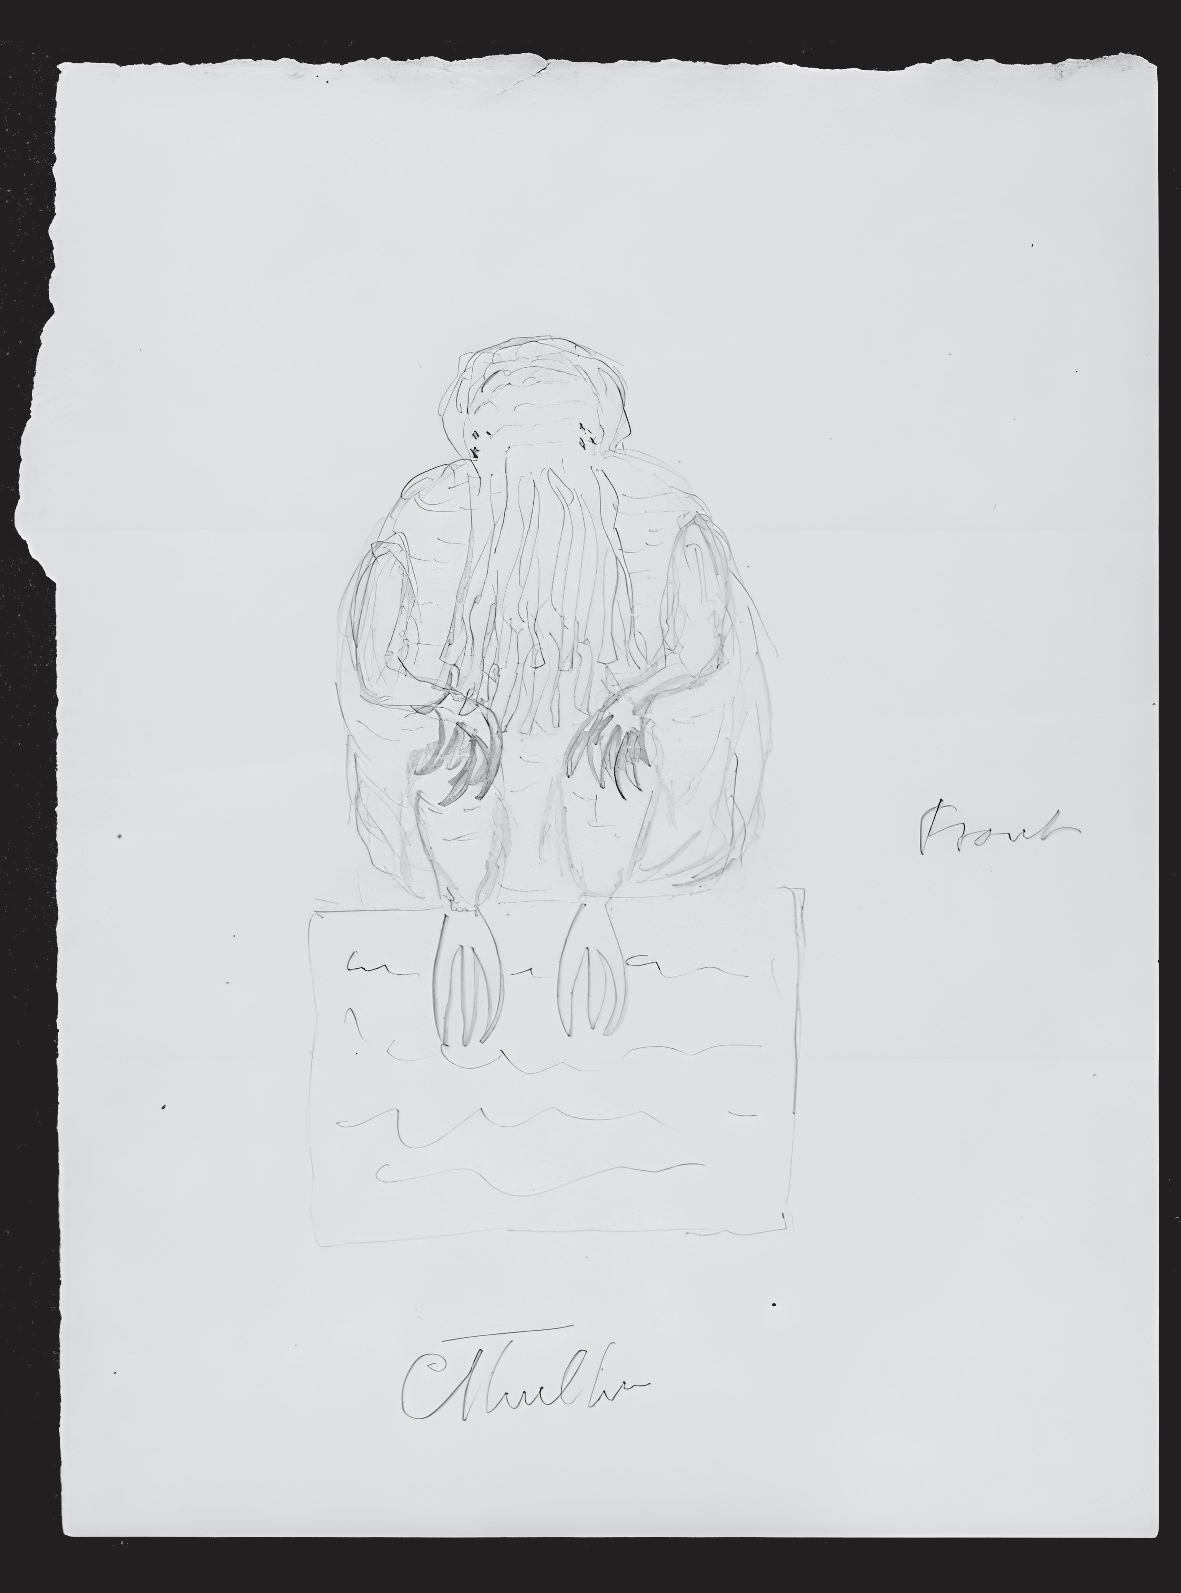
\includegraphics[height=1.03\paperheight]{img/cthulhu4.pdf}};
%\end{tikzpicture}
                    
%\endgroup
%\vfill

\clearpage
\thispagestyle{empty}
\AddToShipoutPicture*{%
  \AtPageCenter{%
    \makebox(0,0){%
      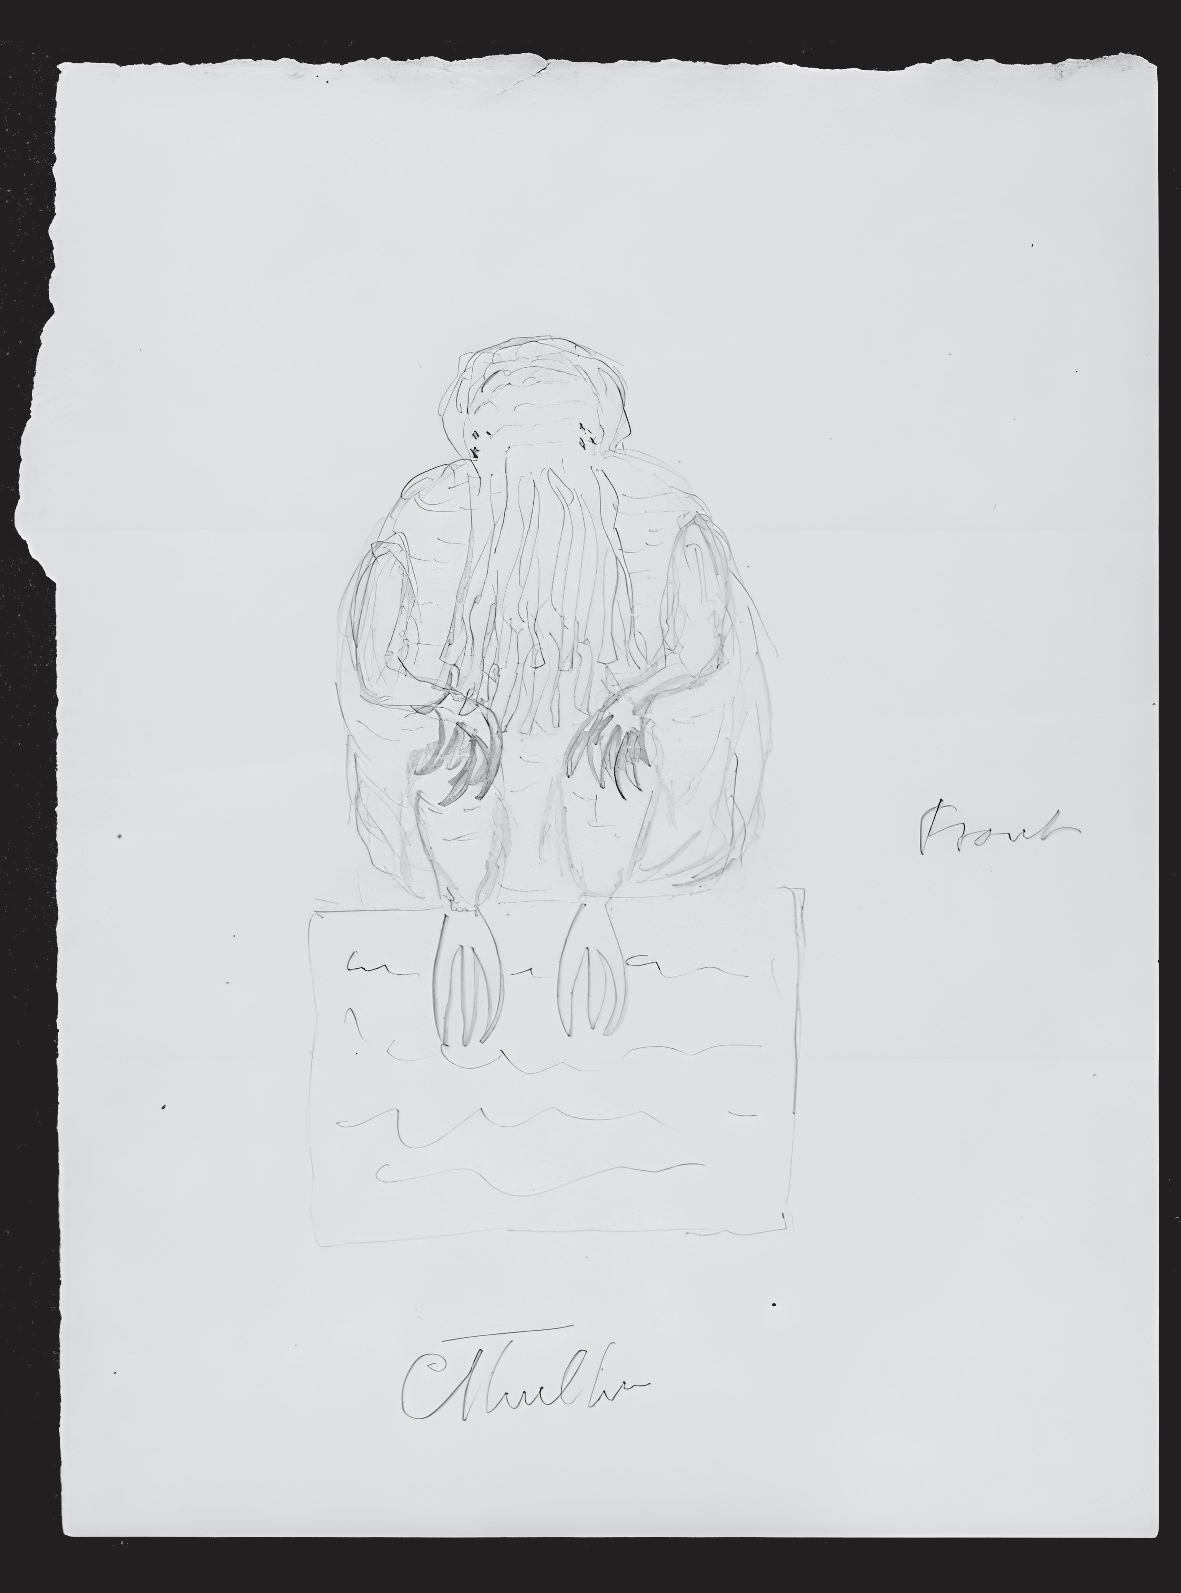
\includegraphics[width=\paperwidth,
                       height=\paperheight,
                       keepaspectratio]{img/cthulhu4.pdf}%
    }%
  }%
}
\null\clearpage % força a emissão da página e evita “vazar” para a próxima
%\pagebreak

\begingroup\thispagestyle{empty}\vspace*{.05\textheight} 

              \formular
              \Huge
              \noindent
              \textbf{O chamado\\ de Cthulhu}
              
              {\brabo\LARGE
              \noindent H.\,P. Lovecraft}

\endgroup
\vfill

\begin{flushleft}
	
\includegraphics[width=.3\textwidth]{img/hedra-audio-qr.png}
\end{flushleft}

\pagebreak